\documentclass[12pt,fullpage,letterpaper]{article}

\newenvironment{proof}{\noindent{\bf Proof:}}{\qed\bigskip}

\newtheorem{theorem}{Theorem}
\newtheorem{corollary}{Corollary}
\newtheorem{lemma}{Lemma} 
\newtheorem{claim}{Claim}
\newtheorem{fact}{Fact}
\newtheorem{definition}{Definition}
\newtheorem{assumption}{Assumption}
\newtheorem{observation}{Observation}
\newtheorem{example}{Example}
\newcommand{\qed}{\rule{7pt}{7pt}}

\newcommand{\assignment}[4]{
\thispagestyle{plain} 
\newpage
\setcounter{page}{1}
\noindent
\begin{center}
\framebox{ \vbox{ \hbox to 6.28in
{\bf CS446: Machine Learning \hfill #1}
\vspace{4mm}
\hbox to 6.28in
{\hspace{2.5in}\large\mbox{Problem Set #2}}
\vspace{4mm}
\hbox to 6.28in
{{\it Handed Out: #3 \hfill Due: #4}}
}}
\end{center}
}


\newcommand{\handout}[3]{
\thispagestyle{plain} 
\newpage
\setcounter{page}{1}
\noindent
\begin{center}
\framebox{ \vbox{ \hbox to 6.28in
{\bf CS446: Machine Learning \hfill #1}
\vspace{4mm}
\hbox to 6.28in
{\hspace{2.5in}\large\mbox{#2}}
\vspace{4mm}
\hbox to 6.28in
{{\it Handed Out: #3 \hfill Name (NetID): \rule[-2pt]{4cm}{0.1pt} }}
}}
\end{center}
}


\newcommand{\assgsoln}[4]{
\thispagestyle{plain} 
\newpage
\setcounter{page}{1}
\noindent
\begin{center}
\framebox{ \vbox{ \hbox to 6.28in
{\bf CS446: Machine Learning \hfill #1}
\vspace{4mm}
\hbox to 6.28in
{\hspace{2.5in}\large\mbox{Problem Set #2 Solutions}}
\vspace{4mm}
\hbox to 6.28in
{{\it Handed Out: #3 \hfill Handed In: #4}}
}}
\end{center}
}


\newcommand{\solution}[4]{
\thispagestyle{plain} 
\newpage
\setcounter{page}{1}
\noindent
\begin{center}
\framebox{ \vbox{ \hbox to 6.28in
{\bf CS446: Machine Learning \hfill #4}
\vspace{4mm}
\hbox to 6.28in
{\hspace{2.5in}\large\mbox{Problem Set #3}}
\vspace{4mm}
\hbox to 6.28in
{#1 \hfill {\it Handed In: #2}}
}}
\end{center}
\markright{#1}
}


\newenvironment{algorithm}
{\begin{center}
\begin{tabular}{|l|}
\hline
\begin{minipage}{1in}
\begin{tabbing}
\quad\=\qquad\=\qquad\=\qquad\=\qquad\=\qquad\=\qquad\=\kill}
{\end{tabbing}
\end{minipage} \\
\hline
\end{tabular}
\end{center}}

\def\Comment#1{\textsf{\textsl{$\langle\!\langle$#1\/$\rangle\!\rangle$}}}


\usepackage{amsmath}
\usepackage{graphicx}
\usepackage{amsfonts}
\usepackage{amssymb}
\usepackage{array,multirow}
\usepackage{rotating}
\oddsidemargin 0in
\evensidemargin 0in
\textwidth 6.5in
\topmargin -0.5in
\textheight 9.0in

\begin{document}

\solution{Hsiang-Wei Hwang}{\today}{2}{Spring 2017}
% Fill in the above, for example, as follows:
% \solution{Joe Smith}{\today}{1}{Fall 2012}

\pagestyle{myheadings}  % Leave this command alone

\begin{enumerate}
\item 
	\begin{itemize}  
		\item[(a)] 
		If choose \texttt{Holiday} as the splitting attribute:
\begin{equation*}
	Gain(H) = Entropy(S) - \sum \frac{|S_v|}{|S|}Entropy(S_v)=
\end{equation*}
\begin{equation*}
	Entropy(S) - \{\frac{21}{50}[-\frac{20}{21}\log_{10}(\frac{20}{21})-\frac{1}{21}\log_{10}(\frac{1}{21})] + \frac{29}{50}[-\frac{15}{29}\log_{10}(\frac{15}{29})-\frac{14}{29}\log_{10}(\frac{14}{29})]\}
\end{equation*}
\begin{equation*}
	 = Entropy(S)-0.209
\end{equation*}
If choose \texttt{Exam Tomorrow} as the splitting attribute:
\begin{equation*}
	Gain(H) = Entropy(S) - \sum \frac{|S_v|}{|S|}Entropy(S_v)=
\end{equation*}
\begin{equation*}
	Entropy(S) - \{\frac{15}{50}[-\frac{10}{15}\log_{10}(\frac{10}{15})-\frac{5}{15}\log_{10}(\frac{5}{15})] + \frac{35}{50}[-\frac{25}{35}\log_{10}(\frac{25}{35})-\frac{10}{35}\log_{10}(\frac{10}{35})]\}
\end{equation*}
\begin{equation*}
	 = Entropy(S)-0.265
\end{equation*}
Thus, I will choose \texttt{Holiday} to get the highest information gain.


		\item[(b)]
		 Replace \textit{Entropy} with \textit{MajorityError}.
For the first layer :\\
Choosing \texttt{Color}:
\begin{equation*}
	Gain = MajorityError(S) - \sum \frac{|S_v|}{|S|}MajorityError(S_v)=
\end{equation*}
\begin{equation*}
	\frac{7}{16} - (\frac{8}{16}\times\frac{3}{8}+ \frac{8}{16}\times\frac{2}{8}) = \frac{7}{16} - \frac{5}{16}
\end{equation*}
Choosing \texttt{Size}:
\begin{equation*}
	Gain = \frac{7}{16} - (\frac{8}{16}\times\frac{3}{8}+ \frac{8}{16}\times\frac{2}{8}) = \frac{7}{16} - \frac{5}{16}
\end{equation*}
Choosing \texttt{Act}:
\begin{equation*}
	Gain = \frac{7}{16} - (\frac{8}{16}\times\frac{2}{8}+ \frac{8}{16}\times\frac{3}{8}) = \frac{7}{16} - \frac{5}{16}
\end{equation*}
Choosing \texttt{Age}:
\begin{equation*}
	Gain = \frac{7}{16} - (\frac{8}{16}\times\frac{2}{8}+ \frac{8}{16}\times\frac{3}{8}) = \frac{7}{16} - \frac{5}{16}
\end{equation*}
All the gains are the same. Choose \texttt{Color} as the splitting attribute.\\
For the second layer at \texttt{Color} = Blue:\\
Choosing \texttt{Size}:
\begin{equation*}
	Gain = \frac{3}{8} - \frac{1}{8}
\end{equation*}
Choosing \texttt{Act}:
\begin{equation*}
	Gain = \frac{3}{8} - \frac{3}{8}
\end{equation*}
Choosing \texttt{Age}:
\begin{equation*}
	Gain = \frac{3}{8} - \frac{3}{8}
\end{equation*}
Choose \texttt{Size} as the splitting attribute.\\
For the second layer at \texttt{Color} = Red:\\
Choosing \texttt{Size}:
\begin{equation*}
	Gain = \frac{2}{8} - \frac{2}{8}
\end{equation*}
Choosing \texttt{Act}:
\begin{equation*}
	Gain = \frac{2}{8} - \frac{2}{8}
\end{equation*}
Choosing \texttt{Age}:
\begin{equation*}
	Gain = \frac{2}{8} - \frac{2}{8}
\end{equation*}
All the gains are the same. Choose \texttt{Size} as the splitting attribute.\\
For the third layer at \texttt{Color} = Blue, \texttt{Size} = Large:\\
Choosing \texttt{Act}:
\begin{equation*}
	Gain = \frac{1}{4} - \frac{1}{4}
\end{equation*}
Choosing \texttt{Age}:
\begin{equation*}
	Gain = \frac{1}{4} - \frac{1}{4}
\end{equation*}
All the gains are the same. Choose \texttt{Act} as the splitting attribute.\\
For the third layer at \texttt{Color} = Blue, \texttt{Size} = small, there is no need to split. The label of the node is F.

For the third layer at \texttt{Color} = Red, \texttt{Size} = Large:\\
Choosing \texttt{Act}:
\begin{equation*}
	Gain = \frac{1}{4} - \frac{1}{4}
\end{equation*}
Choosing \texttt{Age}:
\begin{equation*}
	Gain = \frac{1}{4} - \frac{1}{4}
\end{equation*}
All the gains are the same. Choose \texttt{Act} as the splitting attribute.\\
For the third layer at \texttt{Color} = Red, \texttt{Size} = Small:\\
Choosing \texttt{Act}:
\begin{equation*}
	Gain = \frac{1}{4} - \frac{1}{4}
\end{equation*}
Choosing \texttt{Age}:
\begin{equation*}
	Gain = \frac{1}{4} - \frac{1}{4}
\end{equation*}
All the gains are the same. Choose \texttt{Act} as the splitting attribute. For the forth layer at \texttt{Color} = Blue, \texttt{Size} = Large, \texttt{Act} = Dip, all the labels are Ts. Thus, the label of this node is set as T. For the forth layer at \texttt{Color} = Blue, \texttt{Size} = Large, \texttt{Act} = Stretch. Choose the only attribute, \texttt{Age}, as the splitting attribute. The label of the node \texttt{Age} = Adult is F and the other is T. For the forth layer at \texttt{Color} = Red, \texttt{Size} = Large, \texttt{Act} = Dip, all the labels are Ts. Thus, the label of this node is set as T. For the forth layer at \texttt{Color} = Red, \texttt{Size} = Large, \texttt{Act} = Stretch. Choose the only attribute, \texttt{Age}, as the splitting attribute. The label of the node \texttt{Age} = Adult is F and the other is T. For the forth layer at \texttt{Color} = Red, \texttt{Size} = Small, \texttt{Act} = Dip, all the labels are Ts. Thus, the label of this node is set as T. For the forth layer at \texttt{Color} = Red, \texttt{Size} = Small, \texttt{Act} = Stretch. Choose the only attribute, \texttt{Age}, as the splitting attribute. The label of the node \texttt{Age} = Adult is F and the other is T. Thus, The decision tree:
\begin{verbatim}
if Color = Blue :
  if Size = Large :
    if Act = Dip :
      class = T
    if Act != Dip :
      if Age = Adult :
        class = F
      if Age != Adult :
        class = T  
  if Size != Large :
    class = F
if Color != Blue :
  if Size = Large :
    if Act = Dip :
      class = T
    if Act != Dip :
      if Age = Adult :
        class = F
      if Age != Adult :
        class = T  
  if Size != Large :
    if Act = Dip :
      class = T
    if Act != Dip :
      if Age = Adult :
        class = F
      if Age != Adult :
        class = T      
\end{verbatim}




 		\item[(c)]
		No. Take 1.(b) as an example. when growing the tree, the algorithm sometimes will need to deal with a tie in information gains and generate some redundant nodes without knowing like the node with the splitting attribute \texttt{Size} in the subtree of \texttt{Color} = Red.  
 	\end{itemize}
\item
	\begin{itemize}  
		\item[(a)] 
		I modified the source code, \texttt{FeatureGenerator.java}.\\
1. Modify the feature list.\\
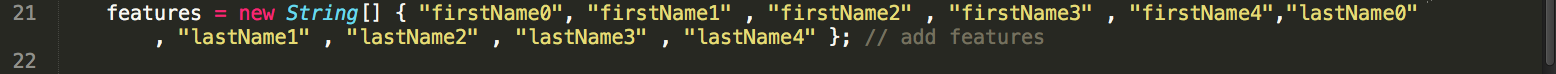
\includegraphics[scale = 0.28]{1.png}\\
2. Add theta as a feature.\\
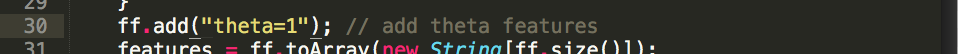
\includegraphics[scale = 0.28]{2.png}\\
3. Change the capacity of the attributes\\
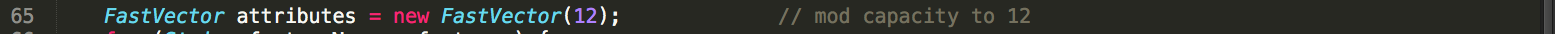
\includegraphics[scale = 0.28]{3.png}\\
4. Extract extra information for new features.\\
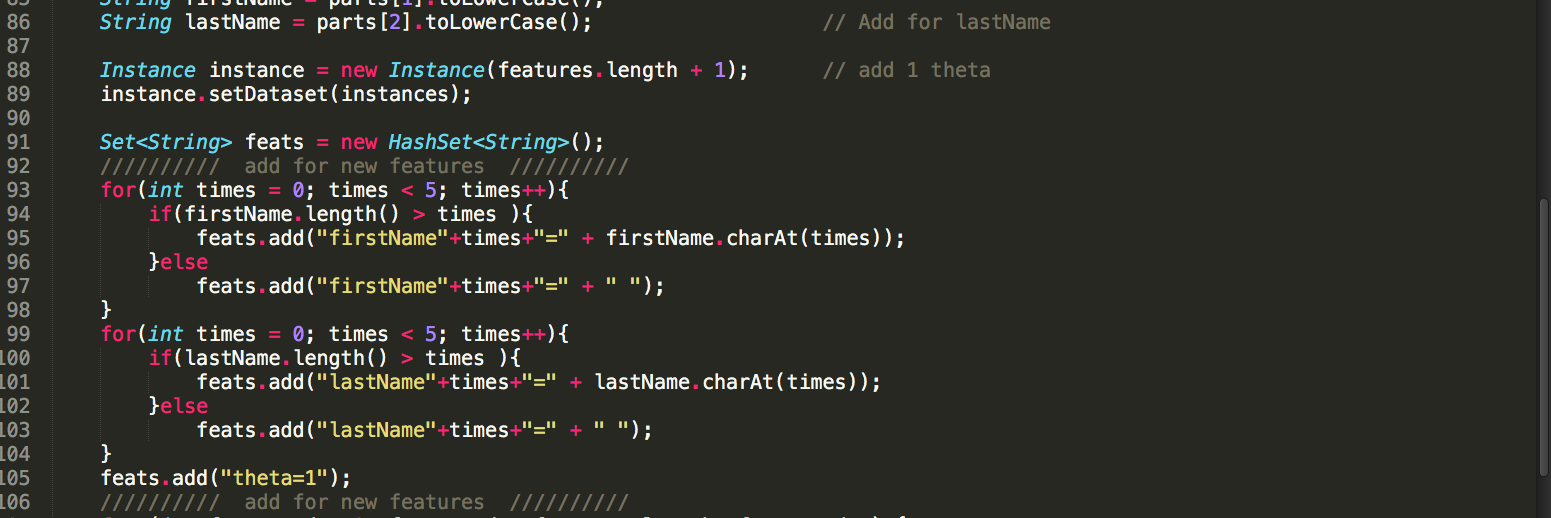
\includegraphics[scale = 0.28]{4.png}\\
		\item[(b)] 
		\textbf{i. Stochastic gradient descent:}\\
We get features from the first 5 alphabets of first name and last name. As mentioned, '1' is added for each feature to represent $\theta$. To fit line, $\vec{w}\vec{x_i}+\theta = y_i$, to the dataset, we use gradient descent method. Assuming the error function $Q(w)$, we could derive the learning method.
\begin{equation*}
	Q(w) = \frac{1}{2}\sum(\vec{w}\vec{x_i}+\theta - y_i)^2
\end{equation*} 
According to the function, $Q(w)$, we modify the weight vector to minimize error function.
\begin{equation*}
	\vec{w'} = \vec{w} - \eta\times \vec{x_i}(\vec{w}\vec{x_i}+\theta - y_i)
\end{equation*}
Keep adjusting the weight vector until error rate of all training set achieving the threshold we set. Then, we sweep different values for threshold and learning rate. The result:
\begin{center}
\begin{tabular}{|c|c|c|c|c|c|}
\hline
\multicolumn{2}{|c|}{} &\multicolumn{4}{|c|}{Learning Rate}  \\ \hline
\multicolumn{2}{|c|}{}  & 0.05 & 0.01 & 0.001 & 0.0001  \\ \hline
\multirow{5}{*}{\rotatebox[origin=c]{90}{Error Threshold}} 
& 0.1 & 0.617 & 0.671 & 0.666 & 0.662 \ \\
&  &  &  &  &  \\\   
& 0.01 & 0.619 & 0.645 & 0.640 & 0.639\  \\
&  &  &  &  &  \\\  
& 0.001 & 0.604 & 0.651 & 0.656 & 0.642\  \\
&  &  &  &  &  \\ \hline
\end{tabular}\\
Coarse sweep of parameters and average accuracy
\end{center}
\begin{center}
\begin{tabular}{|c|c|c|c|c|}
\hline
\multicolumn{2}{|c|}{} &\multicolumn{3}{|c|}{Learning Rate}  \\ \hline
\multicolumn{2}{|c|}{}  & 0.025 & 0.01 & 0.005  \\ \hline
\multirow{5}{*}{\rotatebox[origin=c]{90}{Error Threshold}} 
& 0.25 & 0.624 & 0.613 & 0.617 \  \\
&  &  &  &    \\\  
& 0.1 & 0.676 & 0.671 & 0.675 \  \\
&  &  &  &    \\\  
& 0.05 & 0.680 & 0.672 & 0.683 \  \\ 
&  &  &  &    \\ \hline
\end{tabular}\\
Fine sweep of parameters and average accuracy
\end{center}
According to the table above, we choose learning rate = 0.005 and threshold = 0.05.
\begin{center}
\begin{tabular}{|c|c|c|c|c|c|}
\hline
&\multicolumn{5}{|c|}{Test set}  \\ \hline
 & fold1 & fold2 & fold3& fold4 & fold5 \ \\ \hline
Correct & 45 & 39 & 32& 50 & 35 \ \\ \hline
Wrong & 20 & 18 & 14& 16 & 25 \ \\ \hline
Accuracy & 0.692 & 0.684 &0.696 & 0.758 & 0.583 \\ \hline
\end{tabular}\\
Result of cross validation on SGD
\end{center}
We obtain information from the table$\Rightarrow \bar{x} = 0.683, std = 0.0627$. Two tails with 99\% confidence interval and degree of freedom = 4, T value should be 4.604.
\begin{equation*}
	-4.604\leq \frac{\bar{x} - \mu }{\frac{std}{\sqrt{n}}} \leq 4.604 
\end{equation*}
\begin{equation*}
	\Rightarrow  -4.604\leq \frac{0.683 - \mu }{\frac{0.0627}{\sqrt{5}}} \leq 4.604 
\end{equation*}
\begin{equation*}
	\Rightarrow  0.8118 \ge  {\mu } \ge  0.5534
\end{equation*}
\clearpage
\textbf{ii. Decision tree:}
\begin{center}
\begin{tabular}{|c|c|c|c|c|c|}
\hline
&\multicolumn{5}{|c|}{Test set}  \\ \hline
 & fold1 & fold2 & fold3& fold4 & fold5 \ \\ \hline
Correct & 47 & 40 & 35& 49 & 41 \ \\ \hline
Wrong & 18 & 17 & 11& 17 & 19 \ \\ \hline
Accuracy & 0.723 & 0.702 &0.761 & 0.742 & 0.683 \\ \hline
\end{tabular}\\
Result of cross validation on decision tree
\end{center}
We obtain information from the table$\Rightarrow \bar{x} = 0.7222, std = 0.031$. Two tails with 99\% confidence interval and degree of freedom = 4, T value should be 4.604.
\begin{equation*}
	-4.604\leq \frac{\bar{x} - \mu }{\frac{std}{\sqrt{n}}} \leq 4.604 
\end{equation*}
\begin{equation*}
	\Rightarrow  -4.604\leq \frac{0.7222 - \mu }{\frac{0.031}{\sqrt{5}}} \leq 4.604 
\end{equation*}
\begin{equation*}
	\Rightarrow  -0.064\leq {0.7222 - \mu } \leq 0.064
\end{equation*}
\begin{equation*}
	\Rightarrow  0.7862 \ge  {\mu } \ge  0.6582
\end{equation*}
\textbf{iii. Decision tree of depth 4:}
\begin{center}
\begin{tabular}{|c|c|c|c|c|c|}
\hline
&\multicolumn{5}{|c|}{Test set}  \\ \hline
 & fold1 & fold2 & fold3& fold4 & fold5 \ \\ \hline
Correct & 39 & 39 & 27& 48 & 41 \ \\ \hline
Wrong & 26 & 18 & 19& 18 & 19 \ \\ \hline
Accuracy & 0.600 & 0.684 &0.587 & 0.727 & 0.683 \\ \hline
\end{tabular}\\
Result of cross validation on decision tree of depth 4
\end{center}
We obtain information from the table$\Rightarrow \bar{x} = 0.6564, std = 0.0601$. Two tails with 99\% confidence interval and degree of freedom = 4, T value should be 4.604.
\begin{equation*}
	-4.604\leq \frac{\bar{x} - \mu }{\frac{std}{\sqrt{n}}} \leq 4.604 
\end{equation*}
\begin{equation*}
	\Rightarrow  -4.604\leq \frac{0.6564 - \mu }{\frac{0.0601}{\sqrt{5}}} \leq 4.604 
\end{equation*}
\begin{equation*}
	\Rightarrow  -0.124\leq {0.6564 - \mu } \leq 0.124
\end{equation*}
\begin{equation*}
	\Rightarrow  0.7801 \ge  {\mu } \ge  0.5318
\end{equation*}
\clearpage
\textbf{iv. Decision tree of depth 8:}
\begin{center}
\begin{tabular}{|c|c|c|c|c|c|c|}
\hline
&\multicolumn{6}{|c|}{Test set}  \\ \hline
 & fold1 & fold2 & fold3& fold4 & fold5 & Sum \& Avg\ \\ \hline
Correct & 48 & 41 & 29& 47 & 41 &206\ \\ \hline
Wrong & 17 & 16 & 17& 19 & 19& 88 \ \\ \hline
Accuracy & 0.738 & 0.719 &0.630 & 0.712 & 0.683& 0.701 \\ \hline
\end{tabular}\\
Result of cross validation on decision tree of depth 8
\end{center}
We obtain information from the table$\Rightarrow \bar{x} = 0.6967, std = 0.0421$. Two tails with 99\% confidence interval and degree of freedom = 4, T value should be 4.604.
\begin{equation*}
	-4.604\leq \frac{\bar{x} - \mu }{\frac{std}{\sqrt{n}}} \leq 4.604 
\end{equation*}
\begin{equation*}
	\Rightarrow  -4.604\leq \frac{0.6967 - \mu }{\frac{0.0421}{\sqrt{5}}} \leq 4.604 
\end{equation*}
\begin{equation*}
	\Rightarrow  -0.0867\leq {0.6967 - \mu } \leq 0.0867
\end{equation*}
\begin{equation*}
	\Rightarrow  0.7834 \ge  {\mu } \ge  0.6100
\end{equation*}
\textbf{v. Decision stumps as features \& Stochastic gradient descent:}
\begin{center}
\begin{tabular}{|c|c|c|c|c|c|c|}
\hline
\multicolumn{2}{|c|}{} &\multicolumn{5}{|c|}{Test set}  \\ \hline
\multicolumn{2}{|c|}{} & fold1 & fold2 & fold3& fold4 & fold5 \ \\ \hline
\multirow{3}{*}{\rotatebox[origin=c]{90}{ TD = 4}} 
						& Wrong &25& 20& 19& 16& 16 \ \\ & Correct & 40& 37& 27& 50& 44 \ \\ 
						& Accuracy & 0.615& 0.649& 0.587& 0.758& 0.733\\ \hline
\multirow{3}{*}{\rotatebox[origin=c]{90}{TD = 8}} 
						& Wrong & 22& 16& 17& 15& 19 \ \\ & Correct & 43& 41& 29& 51& 41 \ \\ 
						& Accuracy & 0.662& 0.719& 0.630& 0.773& 0.683\\ \hline
\multirow{3}{*}{\rotatebox[origin=c]{90}{TD = -1}} 
						& Wrong &  21& 17& 21& 19& 20\ \\ & Correct & 44& 40& 25& 47& 40 \ \\ 
						& Accuracy & 0.677& 0.702& 0.543& 0.712& 0.667 \\ \hline						
\end{tabular}\\
Result of cross validation on 100 Decision stumps + SGD with different tree depth
\end{center}
When max tree depth = 4, $\Rightarrow \bar{x} = 0.668, std = 0.074$. We get: 
\begin{equation*}
	0.821 \ge  {\mu } \ge  0.516
\end{equation*}
When max tree depth = 8, $\Rightarrow \bar{x} = 0.693, std = 0.055$. We get: 
\begin{equation*}
	0.806 \ge  {\mu } \ge  0.580
\end{equation*}
When no limitation for max tree depth, $\Rightarrow \bar{x} = 0.660, std = 0.068$. We get: 
\begin{equation*}
	0.800 \ge  {\mu } \ge  0.521
\end{equation*}
After tuning all possible combination parameters, I found that increasing samples when creating decision stumps will largely increase the accuracy. Here, depth of tree = 8, number of trees = 100, we sweep the ratio of removing train data set.
\begin{center}
\begin{tabular}{|c|c|c|c|c|c|c|}
\hline
\multicolumn{2}{|c|}{} &\multicolumn{5}{|c|}{Test set}  \\ \hline
\multicolumn{2}{|c|}{} & fold1 & fold2 & fold3& fold4 & fold5 \ \\ \hline
\multirow{6}{*}{\rotatebox[origin=c]{90}{Use 50\% data }} 
						& Wrong &26& 21& 20& 21& 21 \ \\ 
						&&&&&&  \ \\ 
						& Correct & 39& 36& 26& 45& 39 \ \\ 
						&&&&&&  \ \\ 
						& Accuracy & 0.6& 0.632& 0.565& 0.682& 0.65\\ &&&&&&  \ \\ \hline
\multirow{6}{*}{\rotatebox[origin=c]{90}{Use 60\% data}} 
						& Wrong & 20& 11& 20& 14& 22 \ \\
						&&&&&&  \ \\  
						& Correct & 45& 46& 26& 52& 38 \ \\
						&&&&&&  \ \\  
						& Accuracy & 0.692& 0.807& 0.565& 0.788& 0.633\\ &&&&&&  \ \\ \hline
\multirow{6}{*}{\rotatebox[origin=c]{90}{Use 70\% data}} 
						& Wrong & 23& 18& 16& 10& 16 \ \\ &&&&&&  \ \\ 
						& Correct & 42& 39& 30& 56& 44 \ \\ &&&&&&  \ \\ 
						& Accuracy & 0.646& 0.684& 0.652& 0.848& 0.733\\ &&&&&&  \ \\ \hline
\multirow{6}{*}{\rotatebox[origin=c]{90}{Use 80\% data}} 
						& Wrong & 15& 15& 17& 14& 18 \ \\ &&&&&&  \ \\ 
						& Correct & 50& 42& 29& 52& 42 \ \\ &&&&&&  \ \\ 
						& Accuracy & 0.769& 0.737& 0.660& 0.788& 0.7\\ &&&&&&  \ \\ \hline
\multirow{6}{*}{\rotatebox[origin=c]{90}{Use 90\% data}} 
						& Wrong &  20& 18& 17& 18& 16\ \\ &&&&&&  \ \\ 
						& Correct & 45& 39& 29& 48& 44 \ \\ &&&&&&  \ \\ 
						& Accuracy & 0.692& 0.684& 0.630& 0.727& 0.733 \\ &&&&&&  \ \\ \hline						
\end{tabular}\\
Result of cross validation on 100 Decision stumps of depth 4 + SGD with different sampling ratio
\end{center}
The best case is $\bar{x} = 0.731, std = 0.052$ when randomly sampling 80\% data. \\
99\% confidence interval $\Rightarrow 0.837 \ge  {\mu } \ge  0.624$\clearpage
\textbf{Comparison:}\\
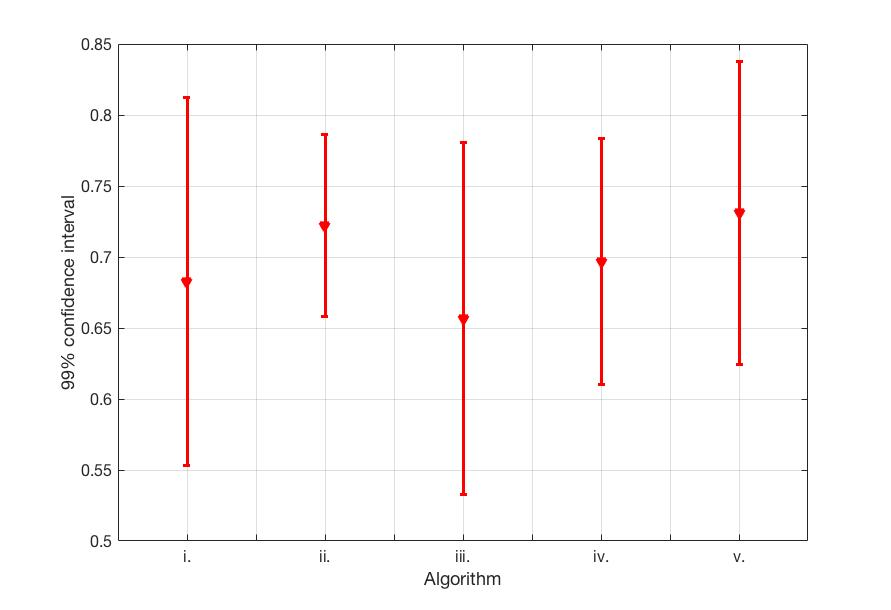
\includegraphics[scale = 0.5]{5.jpg}
According to the 99\% confidence interval we get from t-distribution, the performance of each method is not significantly different from the others. Moreover, the ranking of the first 4 methods is $ii. > iv. > i. > iii.$. However, $v.$ is really hard to compare with others because of the randomization process in it. We could find an average accuracy = 0.731 after adjusting the sampling ratio of training data set to 80\% which is the best of all methods introduced. Thus, roughly speaking, the ranking might be $v. >ii. > iv. > i. > iii.$  

		\clearpage
		\textbf{Trees display for $ii. \mbox{ } iii. \mbox{ } iv.$: }\\
		\textbf{ii. decision tree:}
		\begin{verbatim}
if lastName0=m = 1:
  if firstName2=e = 1: 
    class = +
  if firstName2=e = 0:
    if lastName1=o = 1: 
      class = +
    if lastName1=o = 0:
      if firstName0=p = 1: 
        class = -
      if firstName0=p = 0:
        if firstName0=r = 1: 
          class = -
        if firstName0=r = 0:
          if firstName0=y = 1: 
            class = -
          if firstName0=y = 0:
            if firstName1=u = 1: 
              class = -
            if firstName1=u = 0:
              if lastName3=a = 1:
                if firstName3=r = 1: 
                  class = +
                if firstName3=r = 0: 
                  class = -
              if lastName3=a = 0: 
                class = +
if lastName0=m = 0:
  if lastName1=l = 1:
    if firstName0=d = 1: 
      class = -
    if firstName0=d = 0: 
      class = +
  if lastName1=l = 0:
    if lastName2=l = 1:
      if firstName2=r = 1: 
        class = -
      if firstName2=r = 0:
        if lastName4=n = 1: 
          class = -
        if lastName4=n = 0:
          if firstName2=h = 1: 
            class = -
          if firstName2=h = 0: 
            class = +
    if lastName2=l = 0:
      if lastName2=o = 1:
        if firstName0=b = 1: 
          class = -
        if firstName0=b = 0: 
          class = +
      if lastName2=o = 0:
        if firstName3=f = 1: 
          class = +
        if firstName3=f = 0:
          if lastName4=l = 1:
            if firstName2=h = 1: 
              class = -
            if firstName2=h = 0:
              if lastName0=l = 1: 
                class = -
              if lastName0=l = 0:
                if lastName0=q = 1: 
                  class = -
                if lastName0=q = 0: 
                  class = +
          if lastName4=l = 0:
            if firstName1=o = 1:
              if lastName0=f = 1: 
                class = -
              if lastName0=f = 0:
                if firstName2=e = 1: 
                  class = -
                if firstName2=e = 0:
                  if firstName3=a = 1:
                    if lastName0=h = 1: 
                      class = +
                    if lastName0=h = 0: 
                      class = -
                  if firstName3=a = 0:
                    if firstName2=n = 1: 
                      class = +
                    if firstName2=n = 0:
                      if lastName2=n = 1: 
                        class = +
                      if lastName2=n = 0:
                        if lastName1=a = 1: 
                          class = -
                        if lastName1=a = 0:
                          if firstName3=g = 1: 
                            class = -
                          if firstName3=g = 0: 
                            class = +
            if firstName1=o = 0:
              if lastName0=l = 1:
                if firstName1=a = 1:
                  if firstName0=d = 1: 
                    class = +
                  if firstName0=d = 0: 
                    class = -
                if firstName1=a = 0: 
                  class = +
              if lastName0=l = 0:
                if lastName3=m = 1:
                  if firstName2=r = 1: 
                    class = -
                  if firstName2=r = 0: 
                    class = +
                if lastName3=m = 0:
                  if firstName1=e = 1:
                    if firstName2=n = 1: 
                      class = +
                    if firstName2=n = 0:
                      if firstName2=o = 1:
                        if lastName0=b = 1: 
                          class = -
                        if lastName0=b = 0: 
                          class = +
                      if firstName2=o = 0:
                        if lastName2=r = 1:
                          if firstName0=m = 1: 
                            class = -
                          if firstName0=m = 0: 
                            class = +
                        if lastName2=r = 0: 
                          class = -
                  if firstName1=e = 0:
                    if firstName0=t = 1:
                      if lastName4=e = 1: 
                        class = -
                      if lastName4=e = 0:
                        if lastName0=s = 1: 
                          class = -
                        if lastName0=s = 0: 
                          class = +
                    if firstName0=t = 0:
                      if firstName3=o = 1:
                        if firstName0=a = 1: 
                          class = +
                        if firstName0=a = 0:
                          if firstName0=m = 1: 
                            class = +
                          if firstName0=m = 0: 
                            class = -
                      if firstName3=o = 0:
                        if firstName4=o = 1:
                          if firstName0=s = 1: 
                            class = -
                          if firstName0=s = 0: 
                            class = +
                        if firstName4=o = 0:
                          if lastName0=s = 1:
                            if firstName0=d = 1: 
                              class = +
                            if firstName0=d = 0:
                              if lastName4=h = 1:
                                if firstName0=s = 1: 
                                  class = -
                                if firstName0=s = 0: 
                                  class = +
                              if lastName4=h = 0: 
                                class = -
                          if lastName0=s = 0:
                            if lastName3=l = 1:
                              if firstName0=d = 1: 
                                class = -
                              if firstName0=d = 0: 
                                class = +
                            if lastName3=l = 0: 
                              class = - 
\end{verbatim}
		\clearpage
		\textbf{iii. decision tree of depth 4:}
		\begin{verbatim}
if lastName2=l = 1:
  if firstName2=r = 1: 
    class = -
  if firstName2=r = 0:
    if firstName2=m = 1: 
      class = -
    if firstName2=m = 0: 
      class = +
if lastName2=l = 0:
  if lastName2=o = 1:
    if firstName0=d = 1: 
      class = -
    if firstName0=d = 0:
      if firstName2=l = 1: 
        class = -
      if firstName2=l = 0: 
        class = +
  if lastName2=o = 0:
    if firstName3=f = 1: 
      class = +
    if firstName3=f = 0:
      if lastName0=m = 1:
        if firstName0=n = 1: 
          class = -
        if firstName0=n = 0: 
          class = +
      if lastName0=m = 0:
        if lastName1=l = 1: 
          class = +
        if lastName1=l = 0: 
          class = -
\end{verbatim}
		\textbf{iv. decision tree of depth 8:}
		\begin{verbatim}
if firstName3=f = 1: 
  class = +
if firstName3=f = 0:
  if lastName0=c = 1: 
    class = -
  if lastName0=c = 0:
    if lastName4=l = 1:
      if lastName0=q = 1: 
        class = -
      if lastName0=q = 0: 
        class = +
    if lastName4=l = 0:
      if firstName0=r = 1:
        if firstName1=o = 1: 
          class = +
        if firstName1=o = 0:
          if firstName1=a = 1: 
            class = +
          if firstName1=a = 0:
            if firstName1=e = 1: 
              class = +
            if firstName1=e = 0: 
              class = -
      if firstName0=r = 0:
        if lastName0=m = 1:
          if firstName2=n = 1: 
            class = -
          if firstName2=n = 0:
            if firstName0=p = 1: 
              class = -
            if firstName0=p = 0:
              if lastName2=t = 1:
                if firstName0=t = 1: 
                  class = +
                if firstName0=t = 0: 
                  class = -
              if lastName2=t = 0: 
                class = +
        if lastName0=m = 0:
          if lastName0=l = 1:
            if firstName1=a = 1:
              if firstName0=d = 1: 
                class = +
              if firstName0=d = 0: 
                class = -
            if firstName1=a = 0: 
              class = +
          if lastName0=l = 0:
            if lastName3=m = 1:
              if firstName2=r = 1: 
                class = -
              if firstName2=r = 0: 
                class = +
            if lastName3=m = 0:
              if lastName2=l = 1:
                if firstName2=r = 1: 
                  class = -
                if firstName2=r = 0: 
                  class = +
              if lastName2=l = 0:
                if lastName3=l = 1: 
                  class = +
                if lastName3=l = 0: 
                  class = -

\end{verbatim}
 	\end{itemize}
\end{enumerate}

\end{document}